\begin{frame}
    \begin{exampleblock}{Exercise II}
        \begin{enumerate}
            \item Get the Arduino\textregistered{} \acs{ide} of your choice.
            \item Connect the board to your \acs{pc}.
            \item Connect the board, \acs{led} and resistor on your breadboard.
            \item Control the pin connected to the \acs{led} instead of the on-board \acs{led}.
        \end{enumerate}
    \end{exampleblock}
\end{frame}

\begin{frame}{Breadboards}
    \begin{columns}[t]
        \begin{column}{0.5\textwidth}
            \begin{figure}
                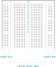
\includegraphics[width=0.9\textwidth]{images/microcontroller/breadboard-expl-1.pdf}
                \caption{Breadboard Layout}
            \end{figure}
        \end{column}
        \begin{column}{0.5\textwidth}
            \begin{figure}
                
\includegraphics[width=0.9\textwidth]{images/microcontroller/breadboard-expl-2.pdf}
                \caption{Breadboard Connections}
            \end{figure}
        \end{column}
    \end{columns}
\end{frame}

% \begin{frame}{Breadboards}
%     \begin{figure}
%         \includegraphics[width=0.9\textwidth]{microcontroller/breadboard-explosion.png}
%         \caption{Breadboard connections}
%     \end{figure}
% \end{frame}

% \begin{frame}{\glsentrydesc{led}}
%     \begin{figure}
%         \includegraphics[width=0.9\textwidth]{microcontroller/leds.png}
%         \caption{\glsentrytext{led} connections}
%     \end{figure}
% \end{frame}

\begin{frame}{\glsentrydesc{led}}
    \begin{figure}
        
\includegraphics[width=0.2\textwidth]{images/microcontroller/led.pdf}
        \caption{\glsentrytext{led} Connections}
    \end{figure}
\end{frame}

% \begin{frame}{Resistors}
%     \begin{figure}
%         \includegraphics[width=0.55\textwidth]{microcontroller/resistor-color-code.png}
%         \caption{Resistors color codes}
%     \end{figure}
% \end{frame}

\begin{frame}{Resistors}
    \begin{figure}
        \resizebox{!}{6cm}{
            \begin{tikzpicture}
                \node[res, scale=0.5, res/second=red, res/third=brown, res/fourth=white, res/sixth=white] (R1) at (0,6) {};
                \node[res, scale=0.5, res/first=blue, res/second=gray, res/third=black, res/fourth=red, res/fifth=silver, res/sixth=white] (R2) at (0,5) {};
                \node[res, scale=0.5, res/first=green, res/second=blue, res/third=black, res/fourth=orange, res/fifth=gold, res/sixth=red] (R3) at (0,4) {};

                \draw[densely dotted] (R1.C1south) -- (R2.C1north);
                \draw[densely dotted] (R2.C1south) -- (R3.C1north);
                \draw[densely dotted] (R3.C1south) -- ++(0.15,-1.5);

                \draw[densely dotted] (R1.C2south) -- (R2.C2north);
                \draw[densely dotted] (R2.C2south) -- (R3.C2north);
                \draw[densely dotted] (R3.C2south) -- ++(0,-1.6);

                \draw[densely dotted] (R2.C3south) -- (R3.C3north);
                \draw[densely dotted] (R3.C3south) -- ++(-0.15,-1.6);

                \node[yshift=-1.8cm,font=\scriptsize] at (R3.C2south) {Digits};

                \draw[densely dotted] (R1.C3south) -- (R2.C4north);
                \draw[densely dotted] (R2.C4south) -- (R3.C4north);
                \draw[densely dotted] (R3.C4south) -- ++(0,-1.2);
                \node[yshift=-1.4cm,xshift=0.2cm,font=\scriptsize] at (R3.C4south) {Multiplier};

                \draw[densely dotted] (R1.C5south) -- (R2.C5north);
                \draw[densely dotted] (R2.C5south) -- (R3.C5north);
                \draw[densely dotted] (R3.C5south) -- ++(0,-0.7);
                \node[yshift=-0.9cm,xshift=0.3cm,font=\scriptsize] at (R3.C5south) {Tolerance};

                \draw[densely dotted] (R3.C6south) -- ++(0,-0.3);
                \node[yshift=-0.5cm,xshift=1.2cm,font=\scriptsize] at (R3.C6south) {Temperature Coefficient};

                \node[xshift=3cm] at (R1.east) {$22\times10^1\longrightarrow\SI{220}{\ohm}\,\pm5\%$};
                \node[xshift=3cm] at (R2.east) {$680\times10^2\longrightarrow\SI{68}{\kilo\ohm}\,\pm10\%$};
                \node[xshift=3cm] at (R3.east) {$560\times10^3\longrightarrow\SI{560}{\kilo\ohm}\,\pm5\%$};

                % Define the colors and their labels
                \def\colors{{"black", "brown", "red", "orange", "yellow", "green", "blue", "violet", "gray", "white"}}
                \def\labelColors{{"white", "black", "black", "black", "black", "black", "white", "white", "white", "black"}}
                \def\colorLabels{{0, 1, 2, 3, 4, 5, 6, 7, 8, 9}}
                \def\multipliers{{"1", "10", "100", "1k", "10k", "100k", "1M", "10M", "100M", "1G"}}
                \def\tolerances{{"N/A", "±1", "±2", "±3", "±4", "±0.5", "±0.25", "±0.1", "±0.05", "N/A"}}
                \def\tempCoefficients{{"N/A", "100", "50", "15", "25", "20", "10", "5", "1", "N/A"}}

                % Draw the color bands
                \foreach \i in {0, ..., 9} {
                        \pgfmathsetmacro{\color}{\colors[\i]}
                        \fill[fill=\color,draw=black] (\i, 0) rectangle ++(1, 1);
                        \draw[] (\i, 0) rectangle ++(1,-3);
                    }

                % Add the digit labels
                \foreach \i in {0, ..., 9} {
                        \pgfmathsetmacro{\label}{\colorLabels[\i]}
                        \pgfmathsetmacro{\labelColor}{\labelColors[\i]}
                        \node[color=\labelColor] at (\i + 0.5, 0.5) {\label};
                    }

                % Add the multiplier labels
                \foreach \i in {0, ..., 9} {
                        \pgfmathsetmacro{\label}{\multipliers[\i]}
                        \node at (\i + 0.5, -0.5) {\scriptsize\label};
                    }

                % Add the tolerance labels
                \foreach \i in {0, ..., 9} {
                        \pgfmathsetmacro{\label}{\tolerances[\i]}
                        \node at (\i + 0.5, -1.5) {\scriptsize\label};
                    }

                % Add the temperature coefficient labels
                \foreach \i in {0, ..., 9} {
                        \pgfmathsetmacro{\label}{\tempCoefficients[\i]}
                        \node at (\i + 0.5, -2.5) {\scriptsize\label};
                    }

                % Draw the labels for digit, multiplier, and tolerance
                \node[anchor=east] at (-0.25, 0.5) {Digit};
                \node[anchor=east] at (-0.25, -0.5) {Multiplier};
                \node[anchor=east] at (-0.25, -1.5) {Tolerance (\%)};
                \node[anchor=east] at (-0.25, -2.5) {Temperature Coefficient (ppm)};

            \end{tikzpicture}
        }
        \caption{Resistor Color Code}
    \end{figure}
\end{frame}

\begin{frame}{Solution: Exercise II}
    \begin{listing}[H]
        \inputsource[fontsize=\fontsize{8}{8}]{c}{arduino/blink-external.c}
        \caption{Solution for Exercise II.}
        \label{lst:arduino:exercise:2:solution}
    \end{listing}
\end{frame}

\begin{frame}{Solution: Exercise II}
    \begin{figure}
        \begin{tikzpicture}
            \ctikzset{bipoles/length=1cm, !vi/.style={no v symbols, no i symbols}, bipole voltage style/.style={text opacity=0}, bipole current style/.style={color=ttw-red}}
            \draw (2,4) node[rp2040] (rp20401) {}
            (rp20401.D2) to ++(1,0) to ++(0,4) to ++(2,0) to ++(0,-1) to [R,name=R,l={$R_1 = \SI{220}{\ohm}$},v=$U_1$,voltage shift=3.5,!vi] ++(0,-1) to [leDo,name=LED,l=$D_1$,v=$U_2$,i=$i$,voltage shift=3.5,!vi] ++(0,-2)
            (rp20401.GNDR) to ++(3,0) to ++(0,1);
            \fixedvlen[0.5cm]{R}{$U_1$}[tw-blue]
            \fixedvlen[0.5cm]{LED}{$U_2$}[tw-blue]
            \iarronly{LED}
        \end{tikzpicture}
        \caption{Circuit for Exercise II}
    \end{figure}
\end{frame}

\begin{frame}{Solution: Exercise II}
    \begin{figure}
        \includegraphics[width=0.35\textwidth]{images/microcontroller/exercises/exercise-2-solution.pdf}
        \caption{Solution for Exercise II.}
    \end{figure}
\end{frame}